\chapter{Test Journal: GPS Variances Test} \label{app:GPSImprovement}

\textbf{Date: TBA}

\subsubsection*{Purpose}
To determine the effectiveness of including base corrections when solving GPS location. Additionally the variance of the GPS is found for the case where the GPS is getting RTK corrections with integer solution, as described in \autoref{app:rtk_gps}.

\subsection*{Equipment}
\begin{itemize}
	\item Emlid Reach RTK GPS connected to the base station as described in Appendix \ref{app:rtk_gps}
  \item Water proof cover.
  \item Active directional GPS antenna with MCX connector.
  \item HTC Desire HD smart phone with access to cellular networks.
\end{itemize}

\subsubsection*{Theory}
By comparing the mean and variance of a GPS with and without base correction, the theoretical improvement in precision and accuracy by including base corrections can be shown.\\
The Emlid Reach module has three different operational modes when receiving corrections from an RTK base. The \emph{Single mode} is when it does not rely on the base. In this mode it works as a regular GPS module. In \emph{RTK Float mode} the module is receiving corrections from the RTK base, but is not using a reliable fix for the integer solution. The last mode is \emph{RTK Fix mode} where it receives RTK correction data with reliable fix for the integer solution. Ideally it should always operate in \emph{RTK Fix mode} to map out the Port of Aalborg withing the requirements.\\
Ideally the correct position of the GPS should be recorded over 42 hours or more by placing the GPS in \emph{Single mode}. This way the average will include a lot of different satellite configurations and no potential bias is added by a base.\\
If the found location is assumed to be correct the accuracy of the proceeding tests can be evaluated with respect to this.\\
For practical reasons this was not prioritized in the project. A 5 hour test was instead performed including all three modes in which the GPS can operate. This is a startup process that the GPS goes through before it receives base corrections and eventually finds a fix for the integer solution.\\
From these results the precision, relevant for the control system, is accessed.
%Under optimal circumstances, this test should be preformed by two similar GPS's at the simultaneously, however it was not a possibility, thus two days with similar weather was chosen as test dates instead.

\subsection*{Procedure}
\begin{enumerate}
  \item Set up the Emlid Reach to log its position in NMEA-format.
  \item Connect the antenna to the Emlid Reach.
	\item Turn on Hotspot on the phone (this should be known to the Emlid Reach module).
	\item Through the reach view app connect the Emlid Reach to the base station.
	\item Water-proof the setup with the cover.
	\item Place the GPS and phone with access to a power outlet and clear sky view.
	\item Wait 5 hours.
	\item Retrieve the setup and extract the data from the logs recorded on the Emlid Reach.
\end{enumerate}

\subsubsection*{Results}

\begin{figure}[H]
  \captionbox
  {
    All three modes of operation are shown here. The Emlid Reach normally goes through all three at startup. However in this case it took longer than observed during testing.
    \label{fig:GPS_2DPlot}
  }
  {
    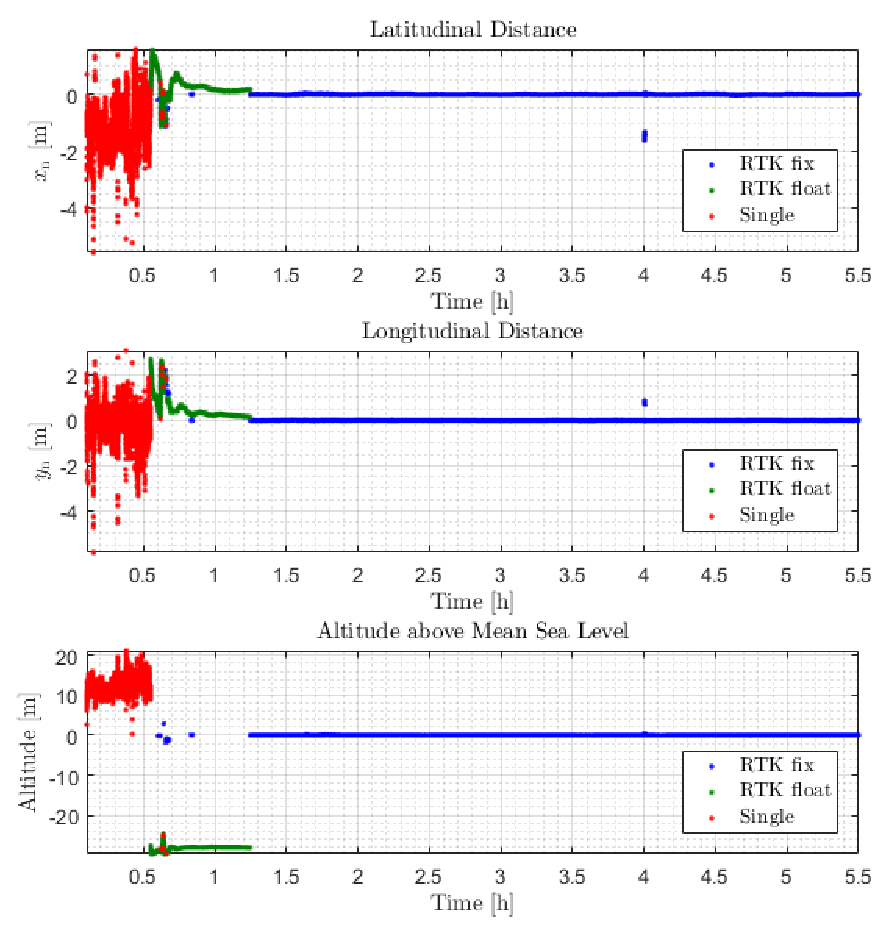
\includegraphics[width=.45\textwidth]{figures/GPS_2DPlot}
  }
  \hspace{5pt}
  \captionbox
  {
    This is the data from \autoref{fig:GPS_2DPlot} plotted in the three dimensions. The $x_n$ and $y_n$ are positions relative to the mean of the Single mode measurements while the altitude is distance above mean sea level.
    \label{fig:GPS_3DPlot}
  }
  {
    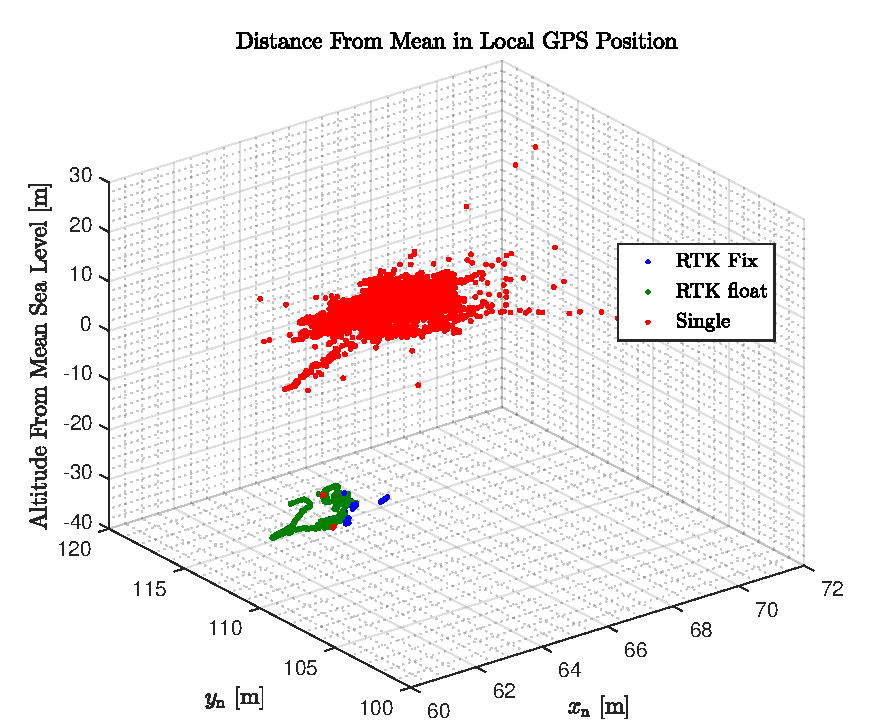
\includegraphics[width=.45\textwidth]{figures/GPS_3DPlot}
    \vspace{1cm}
  }
\end{figure}

In \autoref{fig:GPS_2DPlot} and \autoref{fig:GPS_3DPlot} in altitude is presumed to be caused by the base although, given the limited duration in which single measurements are performed, no reliable conclusion can be drawn. It does however indicate the need for further testing.\\
If the offset is due to bias from the base this can be caused by reflections as described in \ref{app:rtk_gps}.\\
An other thing to note is that the RTK Fix solutions seems very precise compared to the other modes. In the project this is the mode in which the RTK GPS is presumed to operate. For this reason this data is more closely analyzed.

\begin{figure}[H]
  \captionbox
  {
    Here all the data is recorded in \emph{RTK Fix mode} and shown relatie to its own mean to access the precision of the measurements.
    \label{fig:GPS_2DPlot_RTK}
  }
  {
    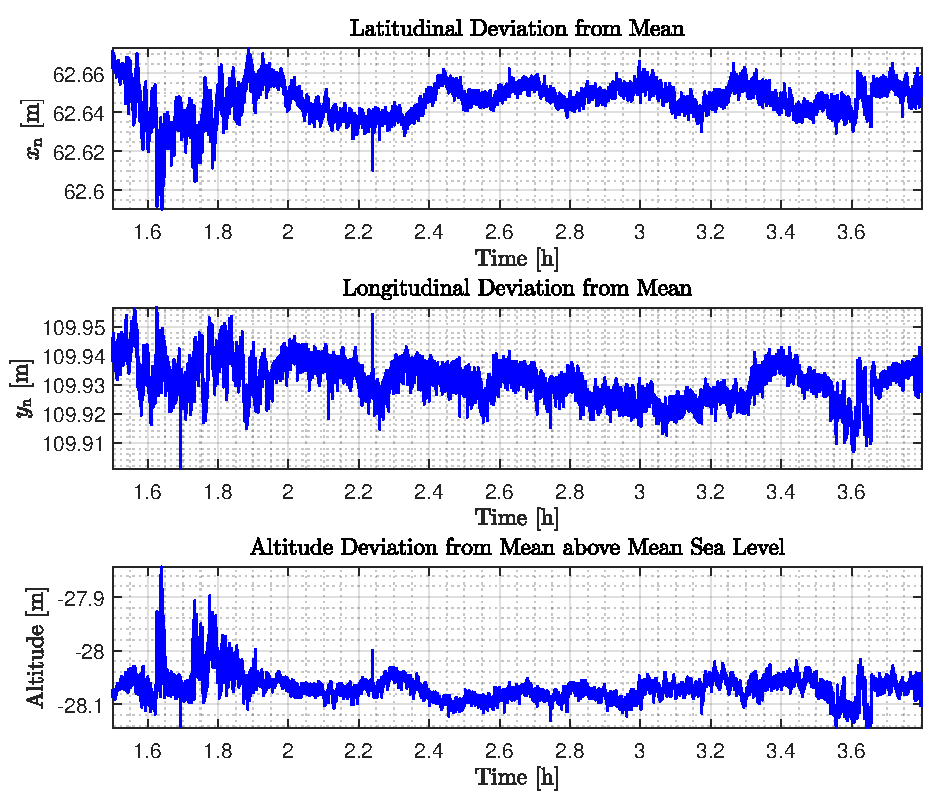
\includegraphics[width=.45\textwidth]{figures/GPS_2DPlot_RTK}
  }
  \hspace{5pt}
  \captionbox
  {
    This is the data from \autoref{fig:GPS_2DPlot_RTK} shown in the three spacial dimensions.
    \label{fig:GPS_3DPlot_RTK}
  }
  {
    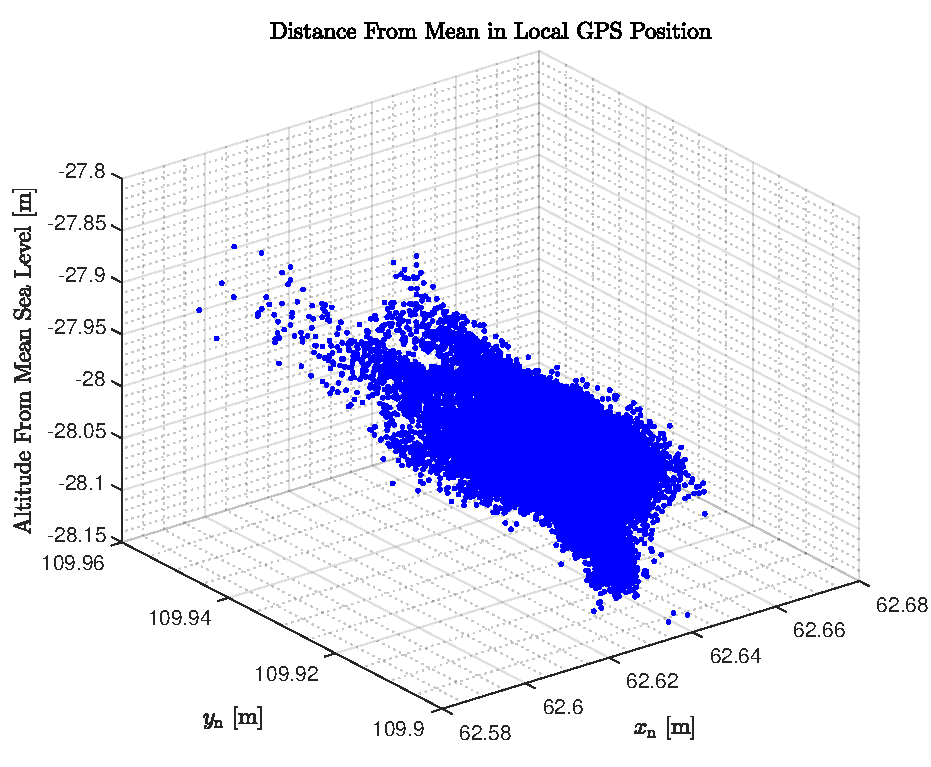
\includegraphics[width=.45\textwidth]{figures/GPS_3DPlot_RTK}
    \vspace{.8cm}
  }
\end{figure}

In \autoref{fig:GPS_2DPlot_RTK} and \autoref{fig:GPS_3DPlot_RTK} the data recorded in \emph{RTK Fix mode} is isolated and plotted around its own mean. The following shows the distribution and presents analysis of the precision of the measurements.

\begin{figure}[H]
  \captionbox
  {
    A histogram of the distance from each point to the mean of the RTK Fix measurements in the $x_n$-$y_n$-plane. The amount of measurements in each bin are scaled as probabilities.
    \label{fig:GPS_RTK_FIX_Histogram}
  }
  {
    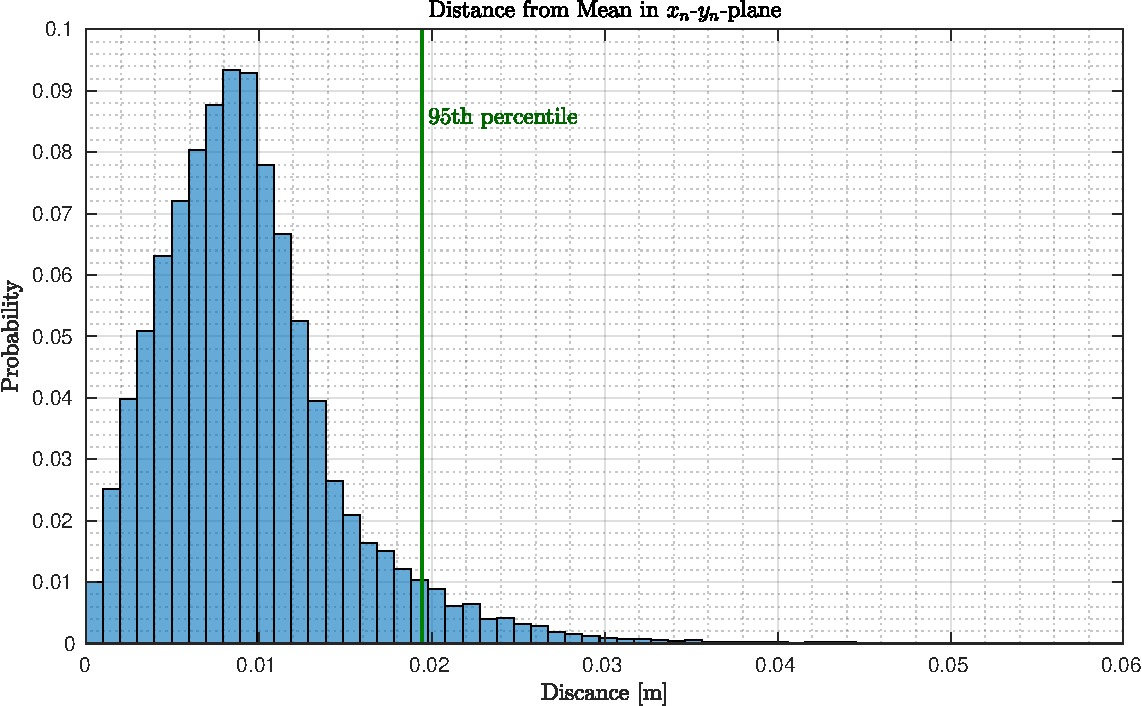
\includegraphics[width=.50\textwidth]{figures/GPS_RTK_Fix_Histogram}
  }
  \hspace{5pt}
  \captionbox
  {
    A histogram of the RTK Fix measurements in the $x_n$-$y_n$-plane. The amount of measurements in each bin are again scaled as probabilities.
    \label{fig:GPS_RTK_FIX_Histogram2}
  }
  {
    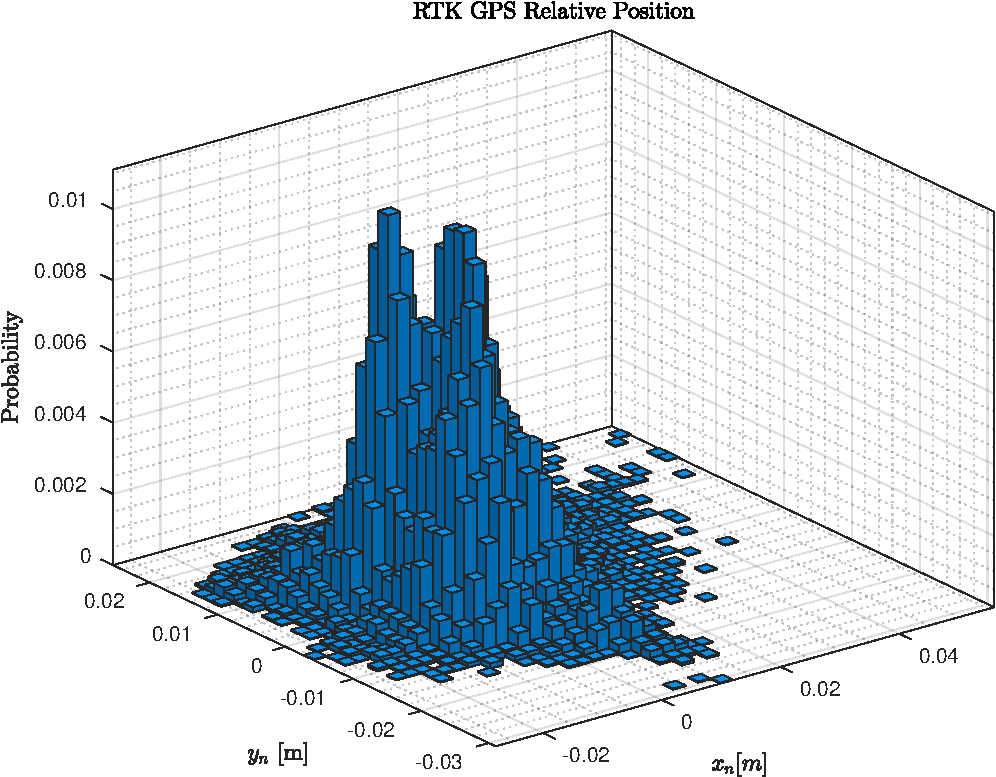
\includegraphics[width=.43\textwidth]{figures/GPS_RTK_Fix_Histogram2}
  }
\end{figure}

In \autoref{fig:GPS_RTK_FIX_Histogram2} the distribution of RTK Fix measurements in the $x_n$-$y_n$-plane relative to their mean is forming a Gaussian distribution. To verify the precision of the measurements shows the planar distances from the data to their mean. The 95th percentile is indicated to show that 95$\%$ of the data has a precision well within the requirement, \textbf{E}, \emph{The THU shall not exceed 30 cm with a 95\% confidence interval.} as stated in \autoref{sec:requirements}.\\
For this requirement to be fulfilled not only the precision but also the accuracy be evaluated. Due to the short duration of the test no reliable conclusion can be drawn. However, there is some indication that the base might cause a bias, see \autoref{fig:GPS_2DPlot_RTK}, and that reflections from nearby buildings might play a role. If further testing supports these claims the base can be moved to a more appropriate location with no immediate obstructions of the signals.


